Are protons unstable?  Few questions within elementary 
particle physics can be posed as simply and at the same time 
have implications as immediate.  In more general terms, the 
apparent stability of protons suggests that baryon number 
is conserved in nature, although no known symmetry 
requires it to be so.  Indeed, baryon number conservation is 
implicit in the formulation of the \dword{sm} Lagrangian, and 
thus observation of \dword{bnv} processes such 
as nucleon decay or neutron-antineutron oscillation 
would be evidence for physics beyond the \dword{sm}.\footnote{Non-perturbative 
effects that involve tunneling between vacua with differing baryon number 
do allow for \dword{bnv} processes within the \dword{sm}, but at rates many orders of 
magnitude below directly observable levels (see, e.g., Ref.~\cite{Nath:2006ut}).}
On the other hand, continued non-observation of \dword{bnv} processes will 
demand an answer to what new symmetry is at play that forbids 
them.
 
Especially compelling is that the observation of \dword{bnv} processes 
could be the harbinger for \dwords{gut}, in which strong, weak and 
electromagnetic forces are unified.  Numerous \dword{gut} models 
have been proposed, each with distinct features.  Yet, \dword{bnv} processes 
are expected on general grounds, and it is a feature of many models 
that nucleon decay channels can proceed at experimentally 
accessible rates (see, e.g., Refs.~\cite{Nath:2006ut,Babu:2013jba} 
and references therein).

The theoretical literature on nucleon decay, and \dword{bnv} processes in general,  
is vast, and has been well summarized in recent 
reviews~\cite{Nath:2006ut,Babu:2013jba}.  
It may be sufficient here to simply note that the 
theoretical motivations for baryon number non-conservation give strong 
arguments for the discovery potential of experimental searches, 
and that the existing array of null results from highly sensitive experiments  
provides hard constraints that models of new physics must abide by.
Some additional theoretical context is provided in Chapter~\ref{ch:nonaccel}.
The remainder of the discussion in this section focuses on the experimental 
landscape so as to illustrate the scientific opportunities for DUNE in \dword{bnv} physics.

\subsection{Experimental Considerations for Nucleon Decay Searches}
\label{subsec:landscape-ndk-expt}

The articulation of early \dword{gut} ideas led to the development of large-scale 
detectors located deep underground dedicated toward the search for proton and \dword{bnv}
bound-neutron decay.  Illustrating the present context, the limits on a subset 
of possible nucleon decay modes, from a succession of sensitive experimental searches, 
are plotted in Fig.~\ref{fig:nucleondecay_exptsummary}.
%
\begin{dunefigure}
[Summary of nucleon decay experimental limits]
{fig:nucleondecay_exptsummary}
{Summary of nucleon decay experimental lifetime limits from past and currently 
running experiments for decays to anti-lepton plus meson final states.  Recently 
reported improvements in limits~\cite{TheSuper-Kamiokande:2017tit} are highlighted, 
indicating the ongoing nature of experimental effort in this area.
The limits shown are 90\% \dword{cl} lower limits on the partial lifetimes, 
$\tau/B$, where $\tau$ is the total mean life and $B$ is the branching fraction. 
Updated from~\cite{Babu:2013jba}.}
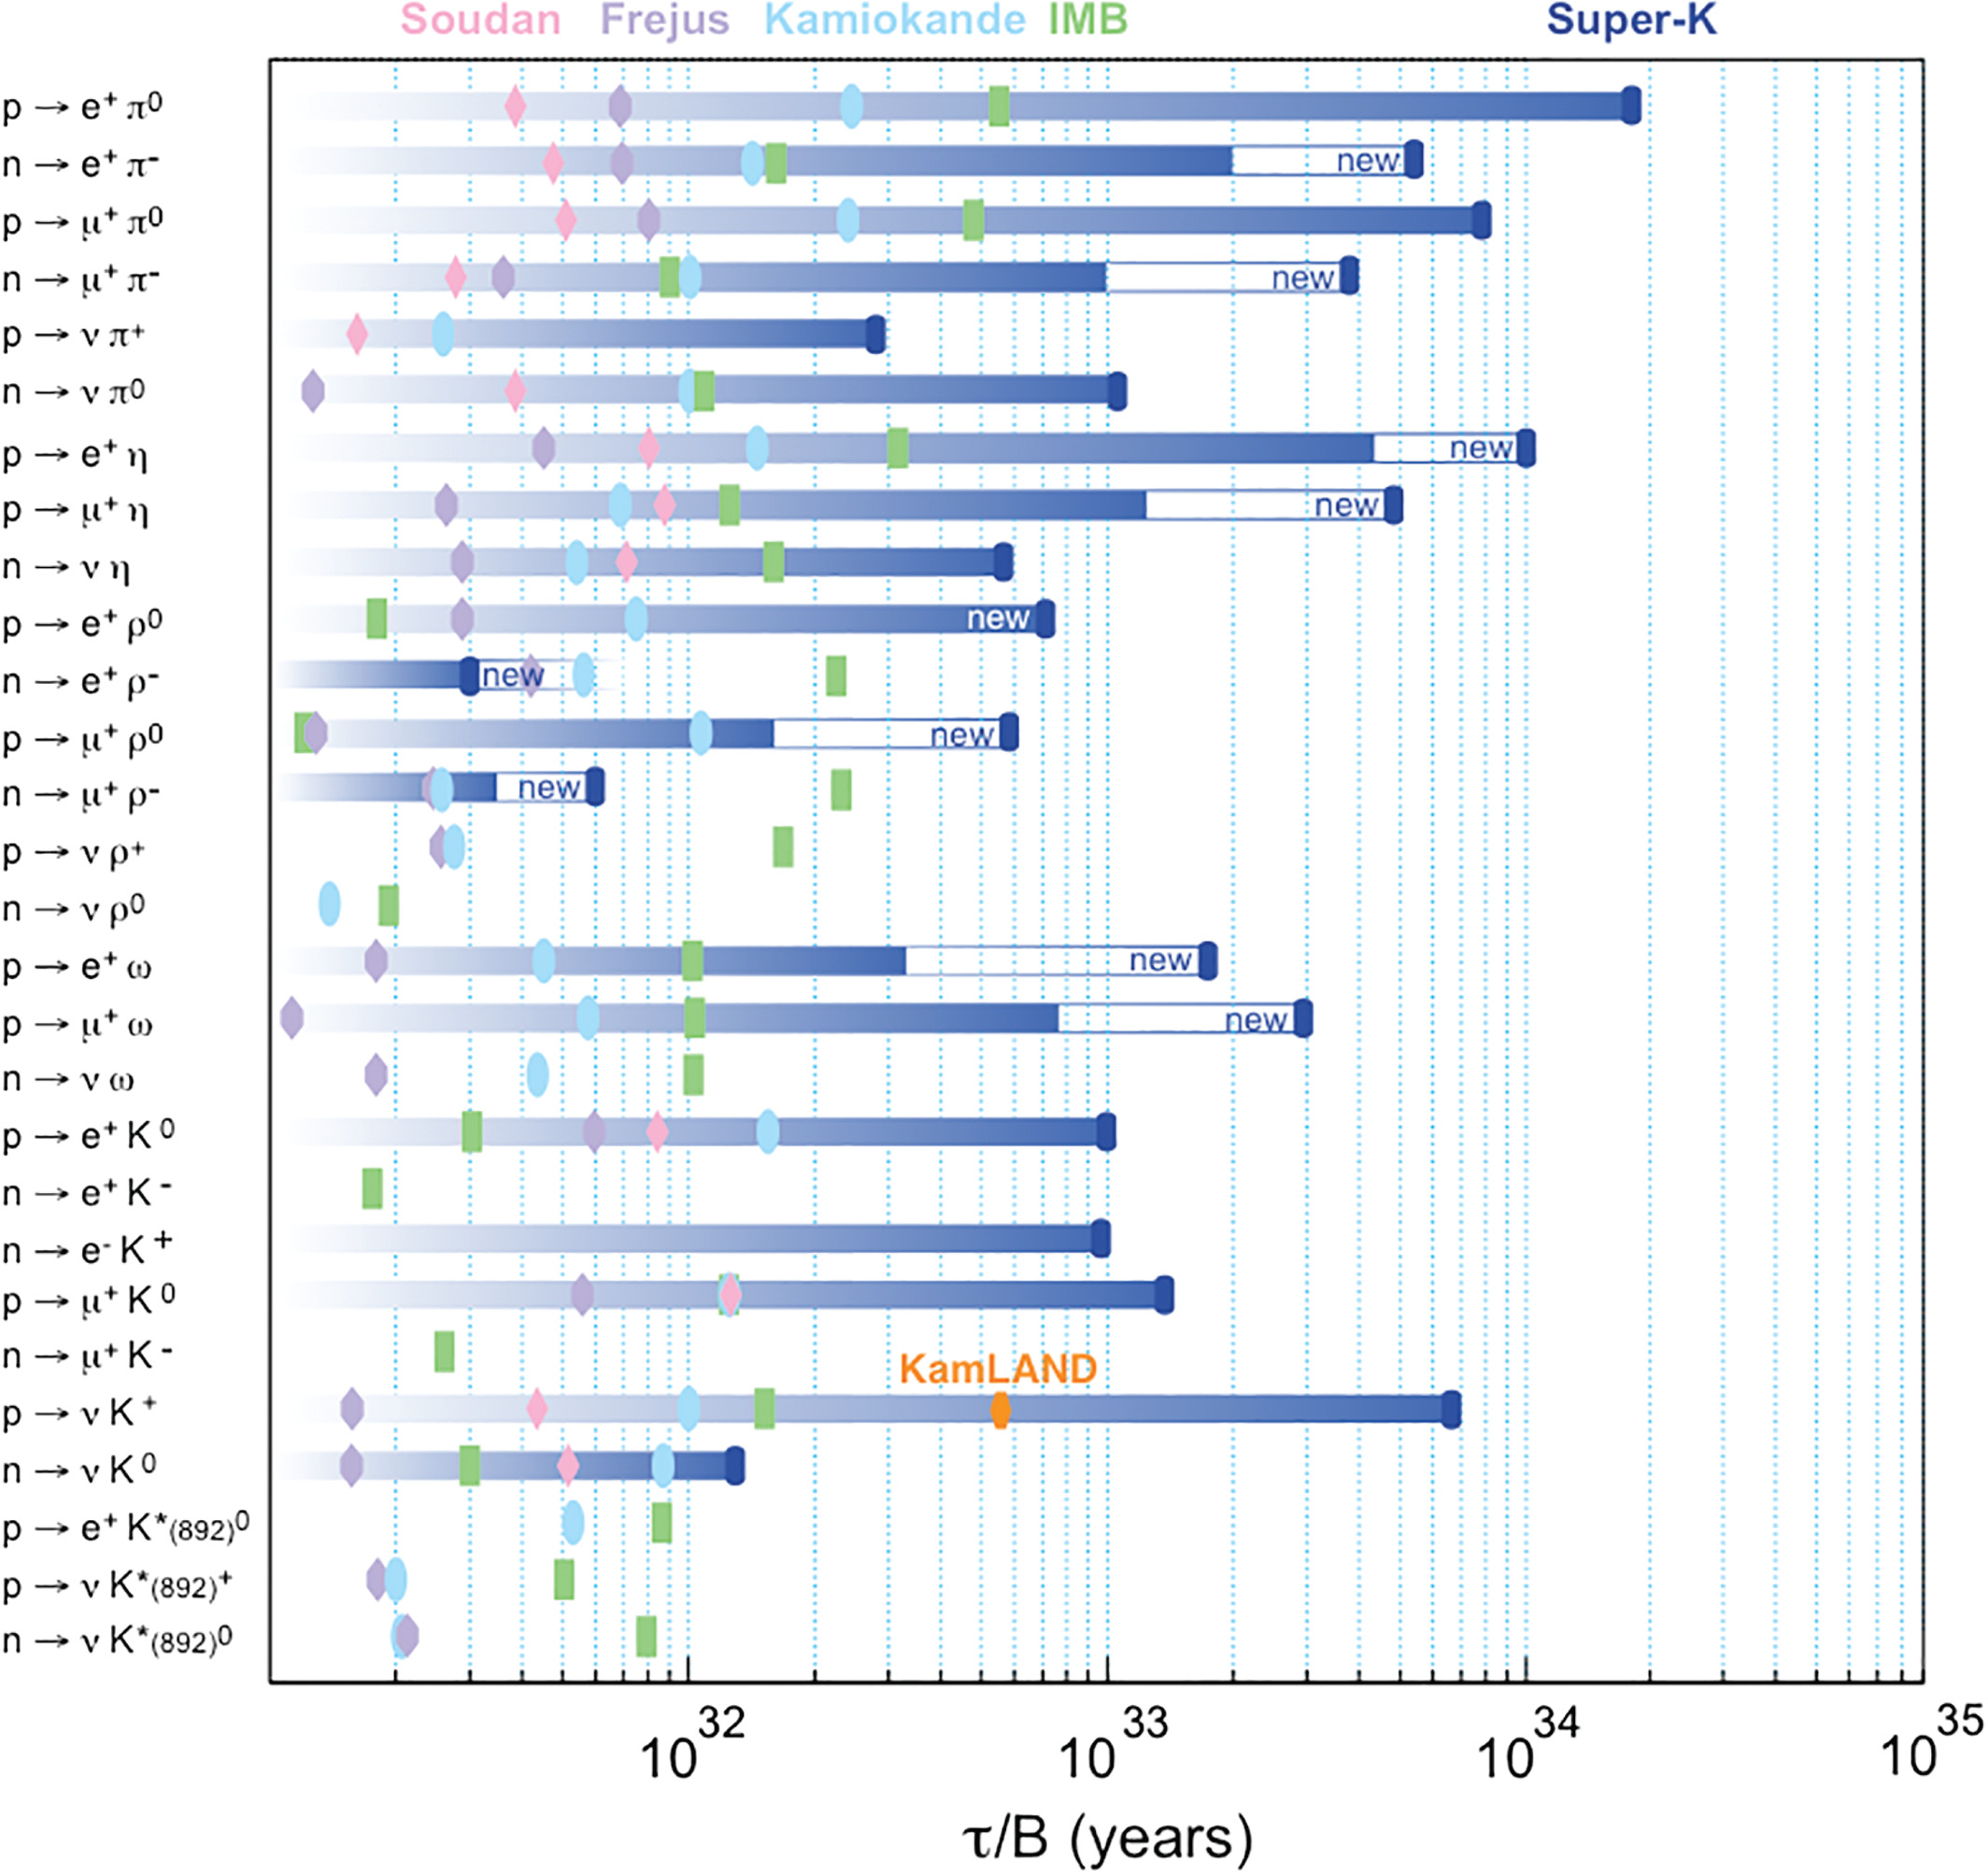
\includegraphics[width=0.8\textwidth]{nucleondecay_exptsummary.jpg}
\end{dunefigure}
%

Particularly sensitive limits have been obtained with water-based Cherenkov ring 
imaging detectors, most notably \superk.  The strengths of this approach include 
the cost-effectiveness of utilizing large volumes of water (\SI{22.5}{\kt} fiducial 
mass in the case of \superk) as a source of nucleons and 
capabilities for particle identification, timing, energy and direction resolution.
The technology is scalable to even larger masses, as in the proposed 
\hyperk~\cite{Abe:2018uyc} experiment, with a \SI{187}{\kt} fiducial mass in its  
single-tank configuration.  The combination of deep underground location with active 
shielding enables rejection of backgrounds from atmospheric muons.  As a result, the 
dominant backgrounds are due to interactions of atmospheric neutrinos, which are suppressed 
by event selection on the distinctive kinematic and signal timing features of
the various nucleon decay channels. 

With published results~(see, e.g., 
Refs.~\cite{Abe:2014mwa,Miura:2016krn,TheSuper-Kamiokande:2017tit})
based on exposures up to \SI{0.32}{\Mtyr}, \superk 
nucleon decay branching ratio sensitivity continues to increase linearly 
with exposure for many channels where background estimates are at the 
one-per-\si{\Mtyr} level.  However, as exposure increases further, the 
rate of improvement will be diminished as backgrounds enter.    
Candidate events are starting to appear~\cite{TheSuper-Kamiokande:2017tit} 
in channels where the estimated background rate exceeds this level.  

With a fiducial mass of \fdfiducialmass{}, DUNE can capitalize on the 
potential for discovery of nucleon decay in channels where backgrounds 
can be reduced below the one-per-\si{\Mtyr} level thanks to the 
excellent imaging, calorimetric and particle identification capabilities 
of the LArTPC for events with 200 to \SI{1000}{\MeV} of deposited energy.  
In a background-free analysis, sensitivity to channels with partial lifetimes 
in the range of $10^{33}$ to a few times $10^{34}$ \si{years} may be achievable, 
depending on event selection efficiency.  The limiting factor for DUNE 
is likely to be the combined impact of nucleon Fermi motion and final state 
interactions of decay hadrons as they escape the argon nucleus.  Detailed 
analyses carried out for several prominent nucleon decay channels are 
described in Chapter~\ref{ch:nonaccel}.

Should nucleon decays occur at rates not far beyond current best limits, 
as predicted in numerous \dword{gut} models, a handful of candidate 
events could be observed by DUNE in a given decay mode.  
Even just one or two candidate events may be 
sufficient on their own to indicate evidence for nucleon decay, 
or provide confirmation 
for an excess above background observed in one of the contemporaneous 
large water or liquid scintillator experiments, e.g., \dword{hyperk}~\cite{Abe:2018uyc}
and JUNO~\cite{Djurcic:2015vqa,An:2015jdp} respectively.
